\documentclass[twoside]{article}
\setlength{\oddsidemargin}{0.25 in}
\setlength{\evensidemargin}{-0.25 in}
\setlength{\topmargin}{-0.6 in}
\setlength{\textwidth}{6.5 in}
\setlength{\textheight}{8.5 in}
\setlength{\headsep}{0.75 in}
\setlength{\parindent}{0 in}
\setlength{\parskip}{0.1 in}

\usepackage{graphicx}
\usepackage{url}

%
% The following commands sets up the lecnum (lecture number)
% counter and make various numbering schemes work relative
% to the lecture number.
%
\newcounter{lecnum}
\renewcommand{\thepage}{\thelecnum-\arabic{page}}
\renewcommand{\thesection}{\thelecnum.\arabic{section}}
\renewcommand{\theequation}{\thelecnum.\arabic{equation}}
\renewcommand{\thefigure}{\thelecnum.\arabic{figure}}
\renewcommand{\thetable}{\thelecnum.\arabic{table}}
\newcommand{\dnl}{\mbox{}\par}

%
% The following macro is used to generate the header.
%
\newcommand{\lecture}[4]{
  \pagestyle{myheadings}
  \thispagestyle{plain}
  \newpage
  \setcounter{lecnum}{#1}
  \setcounter{page}{1}
  \noindent
  \begin{center}
  \framebox{
     \vbox{\vspace{2mm}
   \hbox to 6.28in { {\bf COMPSCI~590S~~~Systems for Data Science
                       \hfill Fall 2016} }
      \vspace{4mm}
      \hbox to 6.28in { {\Large \hfill Lecture #1: #2  \hfill} }
      \vspace{2mm}
      \hbox to 6.28in { {\it Lecturer: #3 \hfill Scribe(s): #4} }
     \vspace{2mm}}
  }
  \end{center}
  \markboth{Lecture {#1}: #2}{Lecture {#1}: #2}
  \vspace*{4mm}
}

%
% Convention for citations is authors' initials followed by the year.
% For example, to cite a paper by Leighton and Maggs you would type
% \cite{LM89}, and to cite a paper by Strassen you would type \cite{S69}.
% (To avoid bibliography problems, for now we redefine the \cite command.)
%
\renewcommand{\cite}[1]{[#1]}

% \input{epsf}

%Use this command for a figure; it puts a figure in wherever you want it.
%usage: \fig{NUMBER}{FIGURE-SIZE}{CAPTION}{FILENAME}
\newcommand{\fig}[4]{
           \vspace{0.2 in}
           \setlength{\epsfxsize}{#2}
           \centerline{\epsfbox{#4}}
           \begin{center}
           Figure \thelecnum.#1:~#3
           \end{center}
   }

% Use these for theorems, lemmas, proofs, etc.
\newtheorem{theorem}{Theorem}[lecnum]
\newtheorem{lemma}[theorem]{Lemma}
\newtheorem{proposition}[theorem]{Proposition}
\newtheorem{claim}[theorem]{Claim}
\newtheorem{corollary}[theorem]{Corollary}
\newtheorem{definition}[theorem]{Definition}
\newenvironment{proof}{{\bf Proof:}}{\hfill\rule{2mm}{2mm}}

% Some useful equation alignment commands, borrowed from TeX
\makeatletter
\def\eqalign#1{\,\vcenter{\openup\jot\m@th
 \ialign{\strut\hfil$\displaystyle{##}$&$\displaystyle{{}##}$\hfil
     \crcr#1\crcr}}\,}
\def\eqalignno#1{\displ@y \tabskip\@centering
 \halign to\displaywidth{\hfil$\displaystyle{##}$\tabskip\z@skip
   &$\displaystyle{{}##}$\hfil\tabskip\@centering
   &\llap{$##$}\tabskip\z@skip\crcr
   #1\crcr}}
\def\leqalignno#1{\displ@y \tabskip\@centering
 \halign to\displaywidth{\hfil$\displaystyle{##}$\tabskip\z@skip
   &$\displaystyle{{}##}$\hfil\tabskip\@centering
   &\kern-\displaywidth\rlap{$##$}\tabskip\displaywidth\crcr
   #1\crcr}}
\makeatother

% **** IF YOU WANT TO DEFINE ADDITIONAL MACROS FOR YOURSELF, PUT THEM HERE:



% Some general latex examples and examples making use of the
% macros follow.

\begin{document}

%FILL IN THE RIGHT INFO.
%\lecture{**LECTURE-NUMBER**}{**DATE**}{**LECTURER**}{**SCRIBE**}
\lecture{10}{Databases: NoSQL, Key-Value stores, Consistent Hashing }{Emery Berger}{Molly McMahon, Janani Krishna}

\section{Concurrency Control}

Concurrency control is important with respect to database management, where concurrency in this context refers to a database with multiple users reading and writing in parallel.It is mostly related to semantics of the database. 

\begin{itemize}
\item Database reads can happen in parallel with no issues
\item Database writes need to be handled in a way that ensures consistency
\end{itemize}

\section{Database Partitioning}

Partitioning or "sharding" refers to distributing one database table among many machines. For example consider a giant table distributed to many machines.\\
\begin{tabular}{c|c|c|c|c}
& ID & Name & Qty & Uid \\
\hline
Machine A & 23000 & Brown & 29 & 1 \\  
 & & .. \\
 \hline
Machine B & 25000 & white & 29 & 2\\
 & & .. \\
 \hline
Machine C & 88000 & Andrew & 70 & 3\\
 & & .. \\
 \hline
\end{tabular} \\\\
The following are different strategies for partitioning:

\subsection{Partitioning by Column}
In this type of partitioning, each column of the table would be stored on a separate machine. 

Cons of this approach:
\begin{itemize}
\item Extent of parallelization is limited to the number of columns
\item A query requiring all columns requires reading from all machines
\end{itemize}

\subsection{Partitioning by Row}
In this type of partitioning, the table is partitioned horizontally; the rows are split into shards which are stored on various machines. This can be done through various hashing strategies.
The possible strategies are:

\subsubsection{Range Partitioning}
To partition the rows, we can sort them by some field (e.g. ID), then define ranges of IDs and map each range to a machine. This approach only works well if the load is well balanced; for example, what happens if your IDs can range 1-1000, but most of your items have ID of 1? In this case, the majority of the rows will map to the same machine. We can attempt to solve this load imbalance by including more fields in our key.NoSQL allows the range partitioning.

\subsubsection{Indexes}
Indexes can be formed based on multiple fields in combination.For example an index can be combination of {(ID,name),qty} etc.This would be feasible only in case of small database.
Potential issues with indexed based approach:
Consider a table of n fields\\
\begin{tabular}{c|c}
No of indexes & fields involved \\
\hline
n & 1  \\  
 \hline
\[ n^2\] & 2 \\
 \hline
\[ n^3\] & 3\\
 \hline
\end{tabular} \\\\
From the table above its clear that as the number of fields involved for creating an index increases the number of indexes increases.The problem will come in case of updates to the index.

\subsubsection{Digest Hashing}
In general hashing has one major issue "Collision", which is unlikely to happen in case of digest hashing.It uses the MD4 algorithm whose hash function is represented as 32 digit hexadecimal number.This particular hashing is most commonly used for integrity checks.

\subsubsection{Hash Partitioning}
To partition a table of entries, we take the entry IDs (or some other field) as keys, compute a hash function on the key, then mod the result by the number of machines to decide which machine to store the entry on.


hash(key) mod N, where N is the number of machines

The motivation of a hash function is to randomly distribute entries onto machines, so that the records will tend to be evenly distributed. This helps with load balancing.

\textbf{Question from a student:}
Consider a query select * from db where qty=10; how does the query work??
\textbf{Answer:} This query is sent to all the machines.In short the entire db is read.

Potential issues with hash partitioning approach:
\begin{itemize}
\item Collisions - by the pigeonhole principle, some keys must hash to the same value
\item Any ordering of the rows (for example, by ID) is destroyed
\item Scalability - bigger hash functions are needed as the number of machines grows. In practice, this isn't really an issue, unless the range of keys is small.
\item Fault tolerance - how to handle a broken machine? If we have replicas, they must all be consistent - ensuring consistency means that machines are doing less useful work. Additionally, in order to keep new entries from hashing to the broken machine, we may need to change the hash function, which would require re-hashing of all the entries. 
\end{itemize}

\subssubsection{Locality Sensitive Hashing (LSH)}
Ensures that entries with similar keys will hash to similar values (not really used much in practice)\\
\begin{figure}[h]
\centering
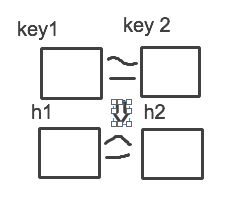
\includegraphics[width=0.5\linewidth]{fig1}
\caption[]{Locality hashing}
\label{cpl}
\end{figure}\\


\subsubsection{Consistent Hashing}
This type of hashing solves the fault tolerance problem. The hash values are arranged in a ring, and machine identifier replicas are randomly distributed around the ring. When a hash value is computed for an entry, the entry is mapped either to the machine at the value's location, or the machine nearest to the value's location. The random distribution of machine identifiers helps with load balancing, so that all entries don't hash to the same machine. When a machine fails, its identifiers are removed from the ring, and all the data that would have hashed to that machine is rehashed to the closest machine left on the ring. In this case, instead of having to compute a new hash function and rehash all the data, we only need to rehash the entries from the failed machine.\\
\begin{figure}[h]
\centering
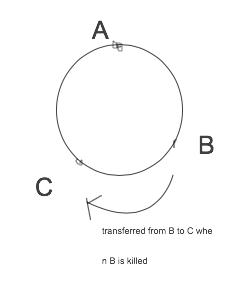
\includegraphics[width=0.5\linewidth]{fig2}
\caption[]{Consistent hashing}
\label{cpl}
\end{figure}\\
 In fig 10.3 when machine B is killed ,some labels like(A,B,D) vitual nodes are added to the virtual space in order to achieve the uniform distribution of data from the machine B.
\begin{figure}[h]
\centering
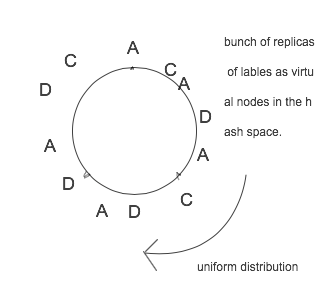
\includegraphics[width=0.5\linewidth]{fig3}
\caption[]{Consistent hashing with uniform distribution}
\label{cpl}
\end{figure}\\

\subsection{Side Note: CDNs}
CDN = Content Distribution Network

CDNs provide content to users by caching it on machines in different geographical locations. Requests are redirected based on the user's location and url hash to one of these machines, so that content can be loaded more quickly. Akamai was one of the first CDNs (this came up because one of the creators of consistent hashing was a co-founder).
\end{document}